\section{Prosess}
\label{chp:prosess}

Prosessen i et forskningsprosjekt kan beskrives som sekvensen av aktiviteter som utføres i løpet av prosjektets varighet \cite{Oates}. Vi vil nå gjøre rede for de metodene og tilnærmingene vi har valgt i vår prosess.

\subsection{Paradigme}
Et paradigme er et sett felles antakelser om, eller måter å tenke på, aspekter av verden \cite{Oates}. Innen samfunnsforskningen fremstår kvalitativ og kvantitativ forskning som to vesentlige tenkemåter, eller paradigmer, når det gjelder hvordan man kan framskaffe eller generere informasjon om samfunnet, for deretter å analysere det \cite{Tjora}. Kvalitativ forskning kan hjelpe forskere å forstå de sosiale og kulturelle kontekstene mennesker lever i \cite{Myers97}, og datamaterialet er ofte rikholdig og detaljert \cite{Oates}. Vi har i dette prosjektet valgt å bruke kvalitative forskningsmetoder for å besvare forskningsspørsmålene.

\subsection{Tidligere arbeid}
Vi fikk innledningsvis i prosjektet utlevert flere artikler som omhandlet vårt forskningsområde av vår veileder. For å definere forskningsspørsmålene i oppgaven, tok vi utgangspunkt i tidligere arbeid gjort av Klemets, Evjemo og Kristiansen \cite{klemets13, Klemets12, KlemetsRedundancy}. Dette ga oss et inntrykk av forskningsområdet og utfordringene knyttet til det eksisterende pasientsignalsystemet. Deretter brukte vi kildene til disse artiklene for å finne utfyllende teori å bygge oppgaven på, samtidig som vår veileder og professor kom med videre forslag til relevant litteratur.  

\subsection{Dokumentstudie}
Ifølge Tjora (2012) er dokumentene en bruker i et dokumentstudie i utganspunktet skrevet for andre formål enn forskning. Slike dokumenter fungerer gjerne som bakgrunns- eller tilleggsdata og kan være casespesifikke eller generelle. Felles for dem er at de er skrevet på et spesielt tidspunkt og sted og gjerne med tanke på spesielle lesere, og det er derfor viktig å sette disse i kontekst.

\noindent
Dokumenter kan være eneste kilde til empiri, eller kun fungere som tilleggsdata \cite{Tjora}. Vi bruker sistnevnte i vår studie, og dokumentene vi har brukt omfatter brukerveiledninger til det eksisterende pasientsignalsystemet, samt strategidokumenter og nettsider tilhørende St.Olavs Hospital. Dette er offentlig tilgjengelige dokumenter som gir relevant og utfyllende informasjon til annen datagenerering.

\subsection{Prototype}
\label{subsec:prototype}
Ifølge Schneiderman og Plaisant (2010) mislykkes mange utviklingsprosjekter i å nå sine mål, i stor grad grunnet dårlig kommunikasjon mellom utviklere og brukere. Suksessfulle utviklere legger derfor stor vekt på å forstå kundens behov og krav. 
Brukersentrert design gir systemer som genererer færre problemer under utviklingen, og lavere vedlikeholdskostnader. De er enklere å lære, gir raskere ytelse og vesentlig mindre feil \cite{mmi}.
Som beskrevet av Mogensen og Trigg (1992), se delkapittel \ref{chp: medvirkning}, kan bruk av kontekstuelle artefakter være nyttig under en deltagende design prosess. En kontekstuell artefakt er en gjenstand medbrakt av fasilitator som brukerene selv setter i kontekst. En prototype kan dermed sies å være en slik artefakt. Dette er i tråd med Gaffney (1999), som anbefaler at man før en deltagende design workshop har vurdert en mulig løsning på forhånd.

\noindent
Prototyping er en velkjent måte å utforske og uttrykke design for interaktive systemer, og er en måte å evaluere løsninger \cite{Houde97}. Houde og Hill (1997) definerer en prototype som enhver representasjon av en designidé, uavhengig av medium. 

\tikzstyle{mybox} = [draw=black, fill=white, very thick,
    rectangle, inner sep=10pt, inner ysep=20pt, rounded corners]
\tikzstyle{fancytitle} =[fill=black, text=white]
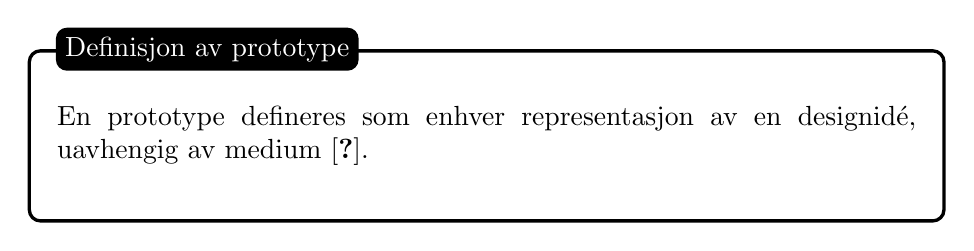
\begin{tikzpicture}
\node [mybox] (box){%
    \begin{minipage}{0.9\textwidth}
      En prototype defineres som enhver representasjon av en designidé, uavhengig av medium \cite{Houde97}.
    \end{minipage}
};
\node[fancytitle, rounded corners, right=10pt] at (box.north west) {Definisjon av prototype};
\end{tikzpicture}%

\noindent
De presenterer tre aspekter ved en prototype; (1) dens rolle, hva gjør den nyttig for brukeren, (2) "look and feel", hva er det brukeren ser, hører og føler når han bruker prototypen, og (3) implementasjon, hvilke teknikker og komponenter utgjør prototypen. Dette er vist i figur \ref{fig: prototype}, hvor skjevheten representerer det faktum at ingen av aspektene, eller dimensjonene, nødvendigvis er viktigere enn de andre.

\begin{figure}[H]
\centering
\includegraphics[scale=1]{prototype.jpg}
\caption{Aspekter ved prototyper}
\label{fig: prototype}
\end{figure}

\noindent
"Rolle"\-prototyper fokuserer på å utforske hvilke funksjoner en bruker kan ha nytte av, og hvilken rolle løsningen vil ha i brukerens liv. Mindre fokus rettes mot hvordan den skal se ut, eller nøyaktig hva som skal til for at den skal fungere. "Look and feel"\-prototyper lages derimot for å undersøke og vise muligheter for hvordan en prototype kan oppleves. "Implementasjon"\-prototyper demonstrerer hvordan en gjenstand kan fungere, og besvarer dermed tekniske spørsmål. Da vår oppgave i stor grad handler om å forstå behov til funksjonalitet, og løsningen vil spille en slags ny rolle i brukerenes liv, ble vårt fokus derfor å lage en prototype som i størst mulig grad utforsker ulike funksjoner.


